\documentclass[tikz,border=2pt]{standalone}
\usepackage{amsmath}
\usepackage{amssymb}
\usepackage{xcolor}

\definecolor{journalink}{HTML}{1F1C18}
\definecolor{journalmuted}{HTML}{8A7F72}
\definecolor{journalaccent}{HTML}{9C2D2D}

\begin{document}
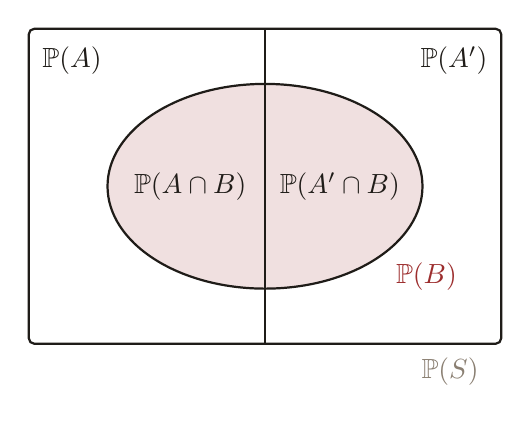
\begin{tikzpicture}[
  x=1cm,
  y=1cm,
  every node/.style={font=\normalsize}
]
  \begin{scope}
    \path[fill=journalaccent, fill opacity=0.15] (1,0) ellipse (2 and 1.3);
  \end{scope}

  \draw[journalink, line width=0.8pt, rounded corners=2pt] (-2,-2) rectangle (4,2);
  \draw[journalink, line width=0.8pt] (1,-2) -- (1,2);
  \draw[journalink, line width=0.8pt] (1,0) ellipse (2 and 1.3);

  \node[journalink] at (-1.45,1.6) {$\mathbb{P}(A)$};
  \node[journalink] at (3.4,1.6) {$\mathbb{P}(A')$};
  \node[journalink] at (0.05,0) {$\mathbb{P}(A\cap B)$};
  \node[journalink] at (1.95,0) {$\mathbb{P}(A'\cap B)$};
  \node[journalaccent] at (3.05,-1.15) {$\mathbb{P}(B)$};
  \node[journalmuted] at (3.35,-2.35) {$\mathbb{P}(S)$};
\end{tikzpicture}
\end{document}
